\documentclass[10pt]{article}
\usepackage[margin=1in]{geometry}
%\addtolength{\oddsidemargin}{-.1in} 
\usepackage{amsmath,amsthm,amssymb}
\usepackage{bm}
\usepackage{enumitem}
\usepackage{array}
\usepackage{lipsum}
\usepackage[]{units}
\usepackage{relsize}
\usepackage{verbatim}

\usepackage{tikz}
\usetikzlibrary{positioning}
\usepackage{graphicx}
\usepackage{xfrac}

\setenumerate{listparindent=\parindent}

\newcommand{\N}{\mathbb{N}}
\newcommand{\Z}{\mathbb{Z}}
\newcommand{\Q}{\mathbb{Q}}
\newcommand{\R}{\mathbb{R}}
\newcommand{\C}{\mathbb{C}}
\newcommand{\D}{\mathbb{D}}

\definecolor{mygray}{rgb}{.8,.8,0.8}

\DeclareMathOperator*{\dom}{dom}
\renewcommand{\bar}{\overline}

\newtheorem*{lem}{Lemma}

\usepackage{fancyhdr}
\pagestyle{fancy}
\lhead{Math 185 (HW 1)}
\chead{Michael Knopf (24457981)}
\rhead{July $6^\text{th}$, 2015}
\lfoot{}
\cfoot{}
\rfoot{}
\renewcommand\headrulewidth{0.4pt}

\begin{document}

\begin{enumerate}

\item Prove that for any pair $z,w$ of complex numbers, the following properties hold:
\begin{itemize}
\item $\bar{z+w} = \bar{z} + \bar{w}$
\item $\bar{zw} = \bar{z}\bar{w}$
\item $|zw| = |z||w|$
\end{itemize}

\begin{proof}
Let $z = a+bi$ and $w = c+di$.
\begin{itemize}
\item $\bar{z+w} = \bar{(a+bi) + (c+di)} = \bar{(a+c) + (b+d)i} = (a+c) - (b+d)i = (a - bi) + (c-di) = \bar{z} + \bar{w}$
\item $\bar{zw} = \bar{(a+bi)(c+di)} = \bar{(ac - bd) + (ad + bc)i} = (ac - bd) - (ad+bc)i = (a-bi)(c-di) = \bar{z}\bar{w}$
\item $|zw| = |(a+bi)(c+di)| = |(ac-bd) + (ad+bc)i| = (ac-bd)^2 + (ad+bc)^2 = a^2 c^2+b^2 c^2+a^2 d^2+b^2 d^2 = (a^2 + b^2)(c^2+d^2) = |a+bi| |c+di| = |z||w|$
\end{itemize}
\end{proof}




\item Prove that the modulus function $\C \rightarrow [0,\infty)$ is continuous.


\begin{lem}
A function $f:X \rightarrow Y$ is continuous if the preimage of every basic open set, for a fixed basis of $Y$, is open.
\end{lem}

\begin{proof}
Let $\mathcal{B}$ be a basis for $Y$, and suppose $f^{-1}(B)$ is open for every $B \in \mathcal{B}$.  Let $U \subseteq Y$ be open.  Then there exists some collection $\mathcal{C} \subseteq \mathcal{B}$ such that $U = \bigcup_{B \in \mathcal{C}} B$.  Therefore,
$$
g^{-1}(U) = g^{-1}(\bigcup_{B \in \mathcal{C}} B) = \bigcup_{B \in \mathcal{C}} g^{-1}(B)
$$
is a union of open sets, and hence open.  So the preimage of every open set is open, thus $f$ is continuous.
\end{proof}
\begin{proof}[Main proof]
The set $\mathcal{B} = \{ [0, b) : b > 0\} \cup \{ (a, b) : a,b \geq 0 \}$ of open balls in $[0,\infty)$ forms a basis for $[0,\infty)$.  The preimage of any open ball of the form $[0,b)$ is the open ball $\{x \in \C : d(0,x) < b \}$ in $\C$, and the preimage of any ball of the form $(a,b)$ is the open annulus $\{ x \in \C : a < d(0,x) < b \}$.  (Clearly, this annulus is open - it is the intersection of two open sets: the open ball of radius $b$ centered at $0$, and the complement of the closed ball of radius $a$ centered at $0$).  Hence, by the lemma, the modulus function is continuous.
\end{proof}

\item Let $p:\C \rightarrow \C$ be a polynomial with real coefficients.  Prove that the roots of $p$ occur in conjugate pairs.

\begin{proof}
Let $p(x) = \sum_{k=0}^n a_k x^k$ for some $a_0, \dots, a_n \in \R$, and suppose that $p(z) = 0$.  Recall that conjugation distributes over addition and multiplication, and also that conjugation is the identity on the real numbers.  Observe that
$$
p(\bar{z}) = \sum_{k=0}^n a_k \bar{z}^k
= \sum_{k=0}^n \bar{a_k} \bar{z^k}
= \bar{\sum_{k=0}^n a_k z^k}
= \bar{p(z)}
=\bar{0}
=0
$$
so $\bar{z}$ is a root of $p$ as well.

Now, suppose that $z \in \C \setminus \R$ has multiplicity $r$ as a root.  We will show by induction on $r$ that $\bar{z}$ has multiplicity $r$ as well.  This is trivial if $r = 0$, since then neither $z$ nor $\bar{z}$ is a root.  Assuming this holds for some $r$, suppose $z$ has multiplicity $r+1$.  We know that $\bar{z}$ is a root, so we may consider the polynomial
$$
q(x) = \frac{p(x)}{(x-z)(x-\bar{z})}.
$$
We know that $z$ is a root of $q(x)$ with multiplicity $r$.  By the inductive hypothesis, $\bar{z}$ is a root with multiplicity $r$ as well.  Clearly, then, $p(x) = (x-z)(x-\bar{z})q(x)$ has $\bar{z}$ as a root with multiplicity $r+1$.
\end{proof}

\item Describe the following sets geometrically and draw a picture of each:
\begin{enumerate}
\item $\{z \in \C : |z+i| \leq 1 \}$
\\
This is the set of all points of distance at most $1$ from the point $-i$.
\item $\{z \in \C : |z-1| = |z-i| \}$
\\
This is the set of points equidistant from $1$ and $i$, which we know from geometry is the perpendicular bisector of the line segment between these two points.
\item $\{z \in \C : |z-4i| + |z+4i| = 10 \}$
\\
An ellipse is the set of points for which the sum of the distances to some two foci is constant.  The major axis must have length 10.  Since $|3-4i| + |3+4i| = 10$, the minor axis has length 6.
\item $\{z \in \C : \frac{1}{z} = \bar{z} \}$
\\
Multiplying both sides by $z$ gives the equation $|z| = 1$.  So this is the unit circle centered at the origin.
\end{enumerate}
\begin{center}
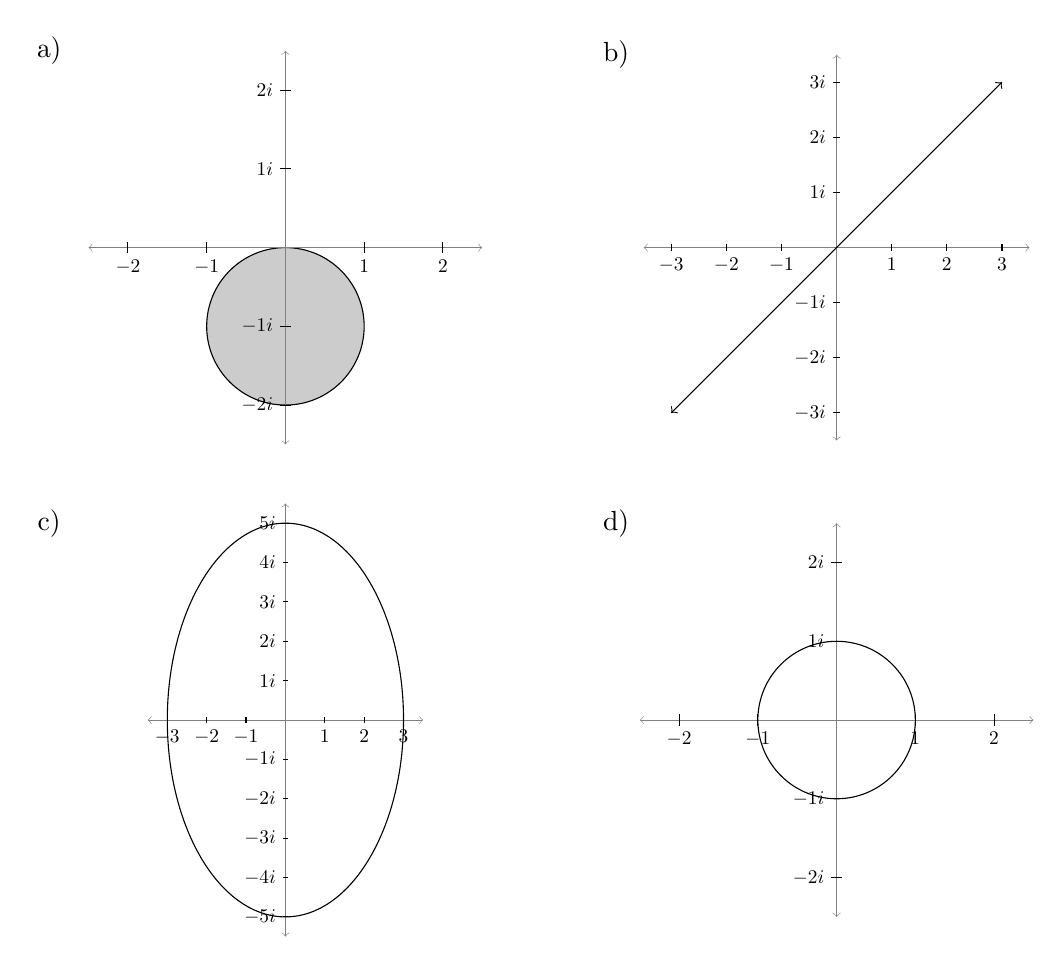
\begin{tikzpicture}

%%%%%%%%%%%%%%% 1 %%%%%%%%%%%%%%%%
\begin{scope}[scale = 1]
\draw [black, fill = mygray] (0,-1) circle [radius=1];
\draw [help lines, <->] (-2.5,0) -- (2.5,0);
\draw [help lines, <->] (0,-2.5) -- (0,2.5);
\foreach \x in {-2,-1,1,2}
	\draw[shift={(\x,0)}] (0pt,2pt) -- (0pt,-2pt) node[below, scale = .7] {$\x$};
\foreach \x in {-2,-1,1,2}
	\draw[shift={(0,\x)}] (2pt,0) -- (-2pt,0) node[left, scale = .7] {$\x i$};
\node at (-3,2.5) {a)};
\node at (-3,-3.5) {c)};
\end{scope}
%%%%%%%%%%%%%%% 2 %%%%%%%%%%%%%%%%

\begin{scope}[xshift = 7cm, scale = .7]
\draw [help lines, <->] (-3.5,0) -- (3.5,0);
\draw [help lines, <->] (0,-3.5) -- (0,3.5);
\foreach \x in {-3,-2,-1,1,2,3}
	\draw[shift={(\x,0)}] (0pt,2pt) -- (0pt,-2pt) node[below, scale = .7] {$\x$};
	%\node [below left, scale = .7] at (\x,0) {$\x$};
\foreach \x in {-3,-2,-1,1,2,3}
	\draw[shift={(0,\x)}] (2pt,0) -- (-2pt,0) node[left, scale = .7] {$\x i$};
\draw [<->] (-3,-3) -- (3,3);
\node at (-4,3.5) {b)};
\node at (-4,-5) {d)};
\end{scope}

%%%%%%%%%%%%%%% 3 %%%%%%%%%%%%%%%%

\begin{scope}[yshift = -6cm, scale = .5]
\draw [help lines, <->] (-3.5,0) -- (3.5,0);
\draw [help lines, <->] (0,-5.5) -- (0,5.5);
\foreach \x in {-3,-2,-1,1,2,3}
	\draw[shift={(\x,0)}] (0pt,2pt) -- (0pt,-2pt) node[below, scale = .7] {$\x$};
	%\node [below left, scale = .7] at (\x,0) {$\x$};
\foreach \x in {-5,-4,-3,-2,-1,1,2,3,4,5}
	\draw[shift={(0,\x)}] (2pt,0) -- (-2pt,0) node[left, scale = .7] {$\x i$};
\draw (0,0) ellipse (3 and 5);
\end{scope}

%%%%%%%%%%%%%%% 4 %%%%%%%%%%%%%%%%

\begin{scope}[xshift = 7cm, yshift = -6cm, scale = 1]
\draw [help lines, <->] (-2.5,0) -- (2.5,0);
\draw [help lines, <->] (0,-2.5) -- (0,2.5);
\foreach \x in {-2,-1,1,2}
	\draw[shift={(\x,0)}] (0pt,2pt) -- (0pt,-2pt) node[below, scale = .7] {$\x$};
	%\node [below left, scale = .7] at (\x,0) {$\x$};
\foreach \x in {-2,-1,1,2}
	\draw[shift={(0,\x)}] (2pt,0) -- (-2pt,0) node[left, scale = .7] {$\x i$};
\draw (0,0) circle [radius = 1];
\end{scope}

\end{tikzpicture}
\end{center}

\item Prove that $\C$ cannot be made into an ordered field.

\begin{proof}
Suppose $(\C, <)$ is an ordered field.  First, assume $i>0$.  This means that $-1 = i \cdot i > 0$, and by the same logic $1 = (-1)(-1) > 0$.  But then we must have $0 = 1 + (-1) > 0$, a contradiction because no element is strictly less than itself in a total ordering.

Next, assume $i < 0$.  Subtracting $i$ from both sides gives $-i > 0$.  Again, we have $(-i)^2 = -1 > 0$.  We have just shown this to be a contradiction.  The only remaining possibility now is $i = 0$, which is absurd.  Therefore, no such ordered field $(\C, <)$ exists.
\end{proof}

\item Let $\D = \{ z \in \C : |z| < 1 \}$.  Fix $w \in \D$ and define $f:\bar{\D} \rightarrow \C$ by
$$
f(z) = \frac{w-z}{1-\bar{w}z}.
$$
Show the following:
\begin{itemize}
\item $f$ maps $\D$ to $\D$ and $\partial \D$ to $\partial \D$.
\item $f$ is a bijection on $\D$.
\item $f$ is holomorphic on $\D$.
\end{itemize}
\end{enumerate}

\begin{proof}
We are given that $|w| < 1$.  To prove that $f$ maps $\D$ to $\D$ and $\partial \D$ to $\partial \D$, we need to show that if $|z| < 1$ then $|f(z)| < 1$ and if $|z| = 1$ then $|f(z)|=1$.  Note that
$$
|f(z)|
=
\left( \frac{w-z}{1-\bar{w}z} \right) \bar{\left(\frac{w-z}{1-\bar{w}z}\right)}
=
\frac{(w-z)(\bar{w} - \bar{z})}{(1-\bar{w}z)(1-w\bar{z})} = \frac{|w| + |z| - (w\bar{z} + \bar{w}z)}{1 + |w||z| - (w\bar{z} + \bar{w}z)}.
$$
If $|z| = 1$ then $f(z) = 1$, since the numerator equals the denominator.  So $f$ maps $\partial \D$ into itself.

To see that $f$ maps $\D$ into itself as well, it suffices to show that if $|z| < 1$ then the numerator is less than the denominator, which is equivalent to showing that $|w| + |z| < 1 + |w||z|$.  This is equivalent to showing
$$
0 < 1 + |w||z| - |w| - |z| = (|w| - 1)(|z|-1).
$$
Given the restriction $|w|, |z| < 1$, this inequality holds since both factors on the right-hand side are negative.

$f$ is its own inverse, so it is a bijection:
$$
f(f(z))
=
\frac{w - \dfrac{w-z}{1-\bar{w}z}}{1 - \bar{w}\dfrac{w-z}{1-\bar{w}z}}
= \frac{(1 - \bar{w}z)w - (w-z)}{(1-\bar{w}z) - \bar{w}(w-z)}
= \frac{w - |w|z - w + z}{1 - \bar{w}z - |w| + \bar{w}z}
= z \left( \frac{1 - \bar{w}}{1 - \bar{w}} \right)
= z.
$$

We will now show that $f$ is holomorphic on $\D$.  The numerator and denominator of $f$ are both linear combinations of holomorphic functions, since $z$ is holomorphic and any constant function is holomorphic.  Also, the denominator is nonzero on $\D$: we know that $|1 - \bar{w}z| \geq ||1| - |\bar{w}z|| > 0$ because $|\bar{w}z| = |w||z| < 1$ for $z,w \in \D$.  Therefore, by the quotient rule, $f$ must be holomorphic on $\D$.
\end{proof}

\end{document}















